\documentclass[a4paper]{report}
\usepackage[utf8]{inputenc}
\usepackage[T1]{fontenc} 
\usepackage[francais]{babel}
\usepackage{graphicx}
\usepackage{geometry}
\usepackage{color}
\usepackage{fancyhdr}
\pagestyle{fancy}
\fancyhf{}
\lhead{2011/2012}
\rhead{IUT Nancy Charlemagne}

\lfoot{Mathieu LEROUX}
\cfoot{Projet tuteuré: Déduplication \\ Licence ASRALL}
\rfoot{\thepage}
\renewcommand{\footrulewidth}{2pt}
\begin{document}
	La déduplication de données est une technique qui permet de minimiser de l'espace de stockage. Elle consiste à ne pas répliquer les données déja existantes sur le disque. Un fichier est décomposé sous forme de blocs de données car des fichiers peuvent avoir des blocs en commum. Le mécanisme de déduplication créé une table avec les indexs de tous les blocs de données des fichiers présent sur le disque. La taille des blocs peut varié selon les mécanismes utilisés mais plus les blocs sont petits, plus il y aura de chance qu'un autre bloc soit idendtique et donc, plus la déduplication sera efficace. En général, cette taille ne dépasse pas les 128ko.
 
 Quand un utilisateur dépose un fichier, le mécanisme crée ses indexs et regarde s'il n'y a pas des blocs déja existant. Si des blocs sont similaires alors une simple référence aux blocs déja existant sera créé. Le schéma ci-dessous montre comment la déduplication fonctionne. Les blocs étant de la meme couleur sont considérés identiques.\\
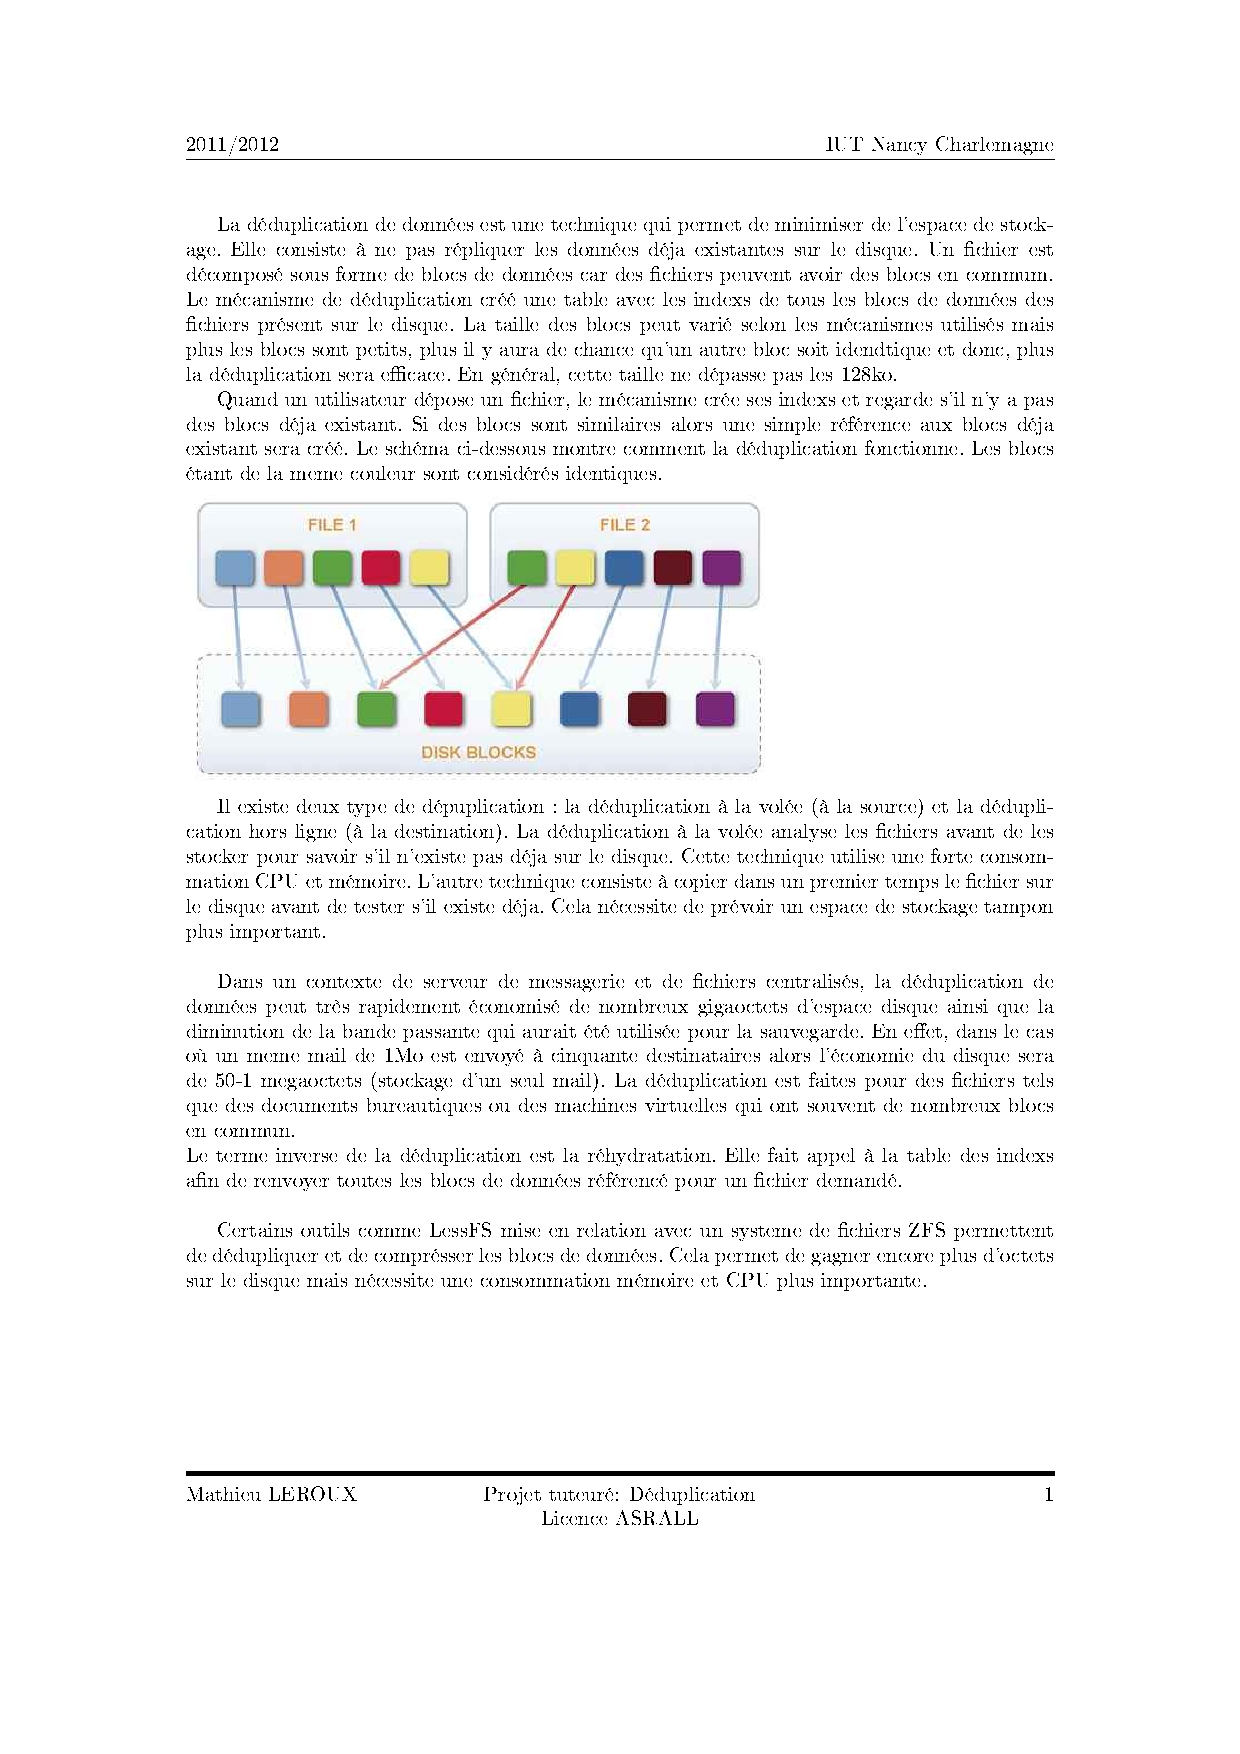
\includegraphics[width=10cm]{deduplication.jpg}

Il existe deux type de dépuplication: la déduplication à la volée (à la source) et la déduplication hors ligne (à la destination). La déduplication à la volée analyse les fichiers avant de les stocker pour savoir s'il n'existe pas déja sur le disque. Cette technique utilise une forte consommation CPU et mémoire. L'autre technique consiste à copier dans un premier temps le fichier sur le disque avant de tester s'il existe déja. Cela nécessite de prévoir un espace de stockage tampon plus important. \\

Dans un contexte de serveur de messagerie et de fichiers centralisés, la déduplication de données peut très rapidement économisé de nombreux gigaoctets d'espace disque ainsi que la diminution de la bande passante qui aurait été utilisée pour la sauvegarde. En effet, dans le cas où un meme mail de 1Mo est envoyé à cinquante destinataires alors l'économie du disque sera de 50-1 megaoctets (stockage d'un seul mail). La déduplication est faites pour des fichiers tels que des documents bureautiques ou des machines virtuelles qui ont souvent de nombreux blocs en commun.\\
Le terme inverse de la déduplication est la réhydratation. Elle fait appel à la table des indexs afin de renvoyer toutes les blocs de données référencé pour un fichier demandé.\\

Certains outils comme LessFS mise en relation avec un systeme de fichiers ZFS permettent de dédupliquer et de comprésser les blocs de données. Cela permet de gagner encore plus d'octets sur le disque mais nécessite une consommation mémoire et CPU plus importante.
\end{document} 
